\documentclass[12pt,fleqn]{book} %taille de la police par défaut, et équations jusitifées à gauche
\usepackage[top=3cm,bottom=3cm,left=3.2cm,right=3.2cm,headsep=10pt,a4paper]{geometry} % marges
\usepackage{xcolor}
\definecolor{enstabGreen}{HTML}{C8D200} 	%vert  	#c8d200 
\definecolor{enstabLightGreen}{HTML}{E9ED99} 	%vert  	#c8d200 
\definecolor{enstabLightBlue}{HTML}{009EE0} %bleu clair 	#009ee0
\definecolor{enstabVeryLightBlue}{HTML}{99D8F3} %bleu clair 	#009ee0
\definecolor{enstabDarkBlue}{HTML}{005C8F}	%bleu foncé 	#005c8f
\definecolor{enstabDarkGrey}{HTML}{333333}	%gris fort 	#333333
\definecolor{enstabLightGrey}{RGB}{48,48,48}	%gris fort 	#333333
\definecolor{enstabParme}{HTML}{8878B2}		%parme 	#8878b2
\definecolor{enstabOrange}{HTML}{F18E00} 	%orange 	#f18e00
\usepackage[colorlinks=true,
        urlcolor=enstabLightBlue,
        anchorcolor=enstabDarkBlue,
        linkcolor=enstabDarkBlue,
        citecolor=enstabDarkGrey,
        pdfauthor={Johan B. C. Engelen},
        pdfkeywords={SVG; LaTeX; Inkscape},
        pdftitle={How to include an SVG image in LaTeX},
        pdfsubject={Describes how to include an SVG image easily in LaTeX using Inkscape}] {hyperref}
\usepackage{url}
\usepackage[utf8]{inputenc} % lettres accentuées
\usepackage[T1]{fontenc}    % Use 8-bit encoding that has 256 glyphs
\usepackage[frenchb]{babel} % Pour le français
\usepackage{cclicenses}     % Licences CC
\usepackage{epigraph}
\usepackage{eso-pic}        % pour une image en fond, page de titre
\usepackage{graphicx}       % Pour inclure des images
\graphicspath{{images/}}    % Où sont les images ?

\usepackage{listings}      % Pour coloriser les codes que vous insérez
\lstset{ %
  backgroundcolor=\color{white},   % choose the background color; you must add \usepackage{color} or 
  basicstyle=\footnotesize\ttfamily,        % the size of the fonts that are used for the code
  breakatwhitespace=false,         % sets if automatic breaks should only happen at whitespace
  breaklines=true,                 % sets automatic line breaking
  captionpos=b,                    % sets the caption-position to bottom
  commentstyle=\color{enstabOrange},    % comment style
  deletekeywords={...},            % if you want to delete keywords from the given language
  escapeinside={\%*}{*)},          % if you want to add LaTeX within your code
  extendedchars=true,              % lets you use non-ASCII characters; for 8-bits encodings only, does not work with UTF-8
  %frame=single,                    % adds a frame around the code
  keepspaces=true,                 % keeps spaces in text, useful for keeping indentation of code (possibly needs columns=flexible)
  keywordstyle=\color{enstabDarkBlue},       % keyword style
  %language=Octave,                 % the language of the code
  morekeywords={*,...},            % if you want to add more keywords to the set
  numbers=left,                    % where to put the line-numbers; possible values are (none, left, right)
  numbersep=8pt,                   % how far the line-numbers are from the code
  numberstyle=\tiny\color{enstabDarkGrey}, % the style that is used for the line-numbers
  rulecolor=\color{black},         % if not set, the frame-color may be changed on line-breaks within not-black text (e.g. comments (green here))
  showspaces=false,                % show spaces everywhere adding particular underscores; it overrides 'showstringspaces'
  showstringspaces=false,          % underline spaces within strings only
  showtabs=false,                  % show tabs within strings adding particular underscores
  stepnumber=5,                    % the step between two line-numbers. If it's 1, each line will be numbered
  stringstyle=\color{enstabParme},     % string literal style
  tabsize=2,                       % sets default tabsize to 2 spaces
  title=\lstname                   % show the filename of files included with \lstinputlisting; also try caption instead of title
}
\usepackage{subcaption}




\usepackage{booktabs}       % pour de jolis tableaux
%\usepackage{fancyhdr}       % pour des entêtes et pieds de pages améliorés.
\usepackage{makeidx}        % requis pour faire les index
\usepackage{glossaries} %requis pour faire le glossaire
     % Ce fichier contient tous les packages nécessaires à la compilation
\makeindex           % donne l'ordre de créer l'index
%\includegraphics[scale=1]{image}
\newacronym{IS}{IS}{Ingénierie Système}
\newacronym{WBS}{WBS}{Work Breakdown Structure}					 % contient les entrées du glossaire
\makeglossaries      % donne l'ordre de créer le glossaire

\begin{document}
\renewcommand{\contentsname}{Sommaire}                % des jolis noms pour la table des matières
%\renewcommand{\bibname}{Références bibliographiques}  % des jolis noms pour les sections bibliographiques
\renewcommand{\glossaryname}{Glossaire}               % et glossaire


%----------------------------------------------------------------------------------------
%	 PAGE DE TITRE
%-----------------------------	-----------------------------------------------------------

\begingroup
\thispagestyle{empty}
\AddToShipoutPicture*{\put(6,5){
\includegraphics[scale=1]{FondTitreSPID}}} % Image background
\begin{center}
\vspace*{2cm}
{\Huge \textsc{\textbf{Rapport d'avancement}}}\\
\vspace*{2cm}
{\Huge \textbf{BMONS}}\par % ACRONYME du projet
\vspace*{2cm}
{\huge Beehive Monitoring System}\par % Intitulé du projet
\end{center}
\vspace*{4cm}

\textbf{\huge Rédigé par :} 

\begin{center}
{
\huge
Alice Danckaers\\
Benoît Raymond\\
Etiene Dalcol\\
Nicolas Van-Nhân Nguyen\\
Tao Zheng\\
Armand Sellier\\
}
\end{center}

\vspace*{1cm}

{\huge \textbf{Sous la direction de :}}\\
\begin{center}
{\huge
Olivier Reynet\\
}
\end{center}
\endgroup


%----------------------------------------------------------------------------------------
%	COPYRIGHT PAGE
%----------------------------------------------------------------------------------------
\newpage
~\vfill
\thispagestyle{empty}

\noindent \bysa 2014 Alice Danckaers, Benoît Raymond, Etiene Dalcol, Nicolas Van-Nhân Nguyen, Tao Zheng and Armand Sellier.\\\\ % Copyright notice

%\noindent \textsc{Published by Publisher}\\ % Publisher

%\noindent \textsc{book-website.com}\\ % URL

\noindent Licensed under the Creative Commons Attribution-ShareAlike 4.0 International Public License.\\ % License information

\noindent \textit{Première impression, décembre 2014} % Printing/edition date

%----------------------------------------------------------------------------------------
%	SOMMAIRE
%----------------------------------------------------------------------------------------
\tableofcontents  % Imprime le sommaire
\cleardoublepage  % pour commencer sur une page impaire

%----------------------------------------------------------------------------------------
%	Préambules
%----------------------------------------------------------------------------------------
\frontmatter      % La partie non numérotée préalable au document principal


\chapter{Remerciements}
\epigraph{La gratitude est non seulement la plus grande des vertus, mais c'est également la mère de tous les autres.}{Emil Cioran}

L'équipe du projet BMONS (BeeHive Monitoring System) souhaiterait remercier monsieur O.Reynet, responsable de l'UV 3.4 et auteur de notre sujet ainsi que notre encadrant IS, monsieur B.CLEMENT pour leurs conseils, leur soutient et leur disponibilité. Ils ont su nous guider tout au long du projet notamment sur le plan technique et architectural de notre système. \\

Nous tenons également à remercier monsieur F.Singhoff, professeur à l'université de Bretagne Occidentale à Brest dans le domaine des systèmes embarqués et apiculteur, qui a accepté de prendre part à notre projet en tant que "client" en partageant ainsi son expérience de l'apiculture. Il a aussi mis à notre disposition une de ses ruches afin que nous puissions nous rendre compte des dimensions et de l'espace disponible pour installer notre système.
       
 

\chapter{Préambule}
\epigraph{Le chemin est long du projet à la chose.}{Molière}

\section{Comment compiler ce document ?}

Un document \LaTeX peut se compiler au travers d'un IDE (TexSutdio, TeXMaker par exemple).
Le répertoire de ce document contient également un Makefile qui permet de compiler simplement en ligne de commande. 
La fabrication du glossaire et de l'index est prise en charge par ce Makefile.
Pour l'utiliser, il suffit d'ouvrir un terminal, de se placer dans le répertoire du document puis d'invoquer la commande \texttt{make}. 


Voici les différentes cibles disponibles pour ce Makefile :
\begin{verbatim}
make                - contruit le document
make all            - contruit le document
make index          - contruit l'index
make glossaire      - contruit le glossaire
make bib            - contruit la bibliographie
make pdf            - contruit le document PDF
make clean          - supprime les fichiers LaTeX intermédiaires
make clean-all      - supprime tous les fichiers générés par la compilation
make help           - cette information
\end{verbatim}


\section{Références internes}

Les références internes sont des renvois vers des figures, des tableaux ou des sections du rapport.
\LaTeX introduit un mécanisme simple pour établir ce genre de référence, via les commandes \texttt{\textbackslash label} et \texttt{\textbackslash ref}. 
La première sert à définir une ancre dans le document, la seconde à la citer.
Voici par exemple une référence interne vers la section intitulée \textit{Approche Top-Down} (cf. section  \ref{sec:top-down}). Ce renvoi est le résultat de la commande \texttt{\textbackslash ref\{sec:top-down\}}. Si vous vous rendez dans le corps de cette section, vous y trouverez le label en question \texttt{\textbackslash label\{sec:top-down\}}. 

\subsection{Tableaux et figures}
Les figures  et les tableaux  sont référencés de la même la manière (cf. figure \ref{fig:gomboc} et tableau \ref{tab:exemple}). \index{Table} \index{Figure}

\begin{table}[h]
\centering
\begin{tabular}{lll}
\toprule
\textbf{Algorithmes} & \textbf{Performance (s)} & \textbf{Gain (dB)}\\
\midrule
Algorithme 1 & 0.0003262 & 0.562 \\
Algorithme 2 & 0.0015681 & 0.910 \\
Algorithme 3 & 0.0009271 & 0.296 \\
\bottomrule
\end{tabular}
\caption{\label{tab:exemple}Performances et gains des algorithmes envisagés.}
\end{table}

\begin{figure}[h]
\centering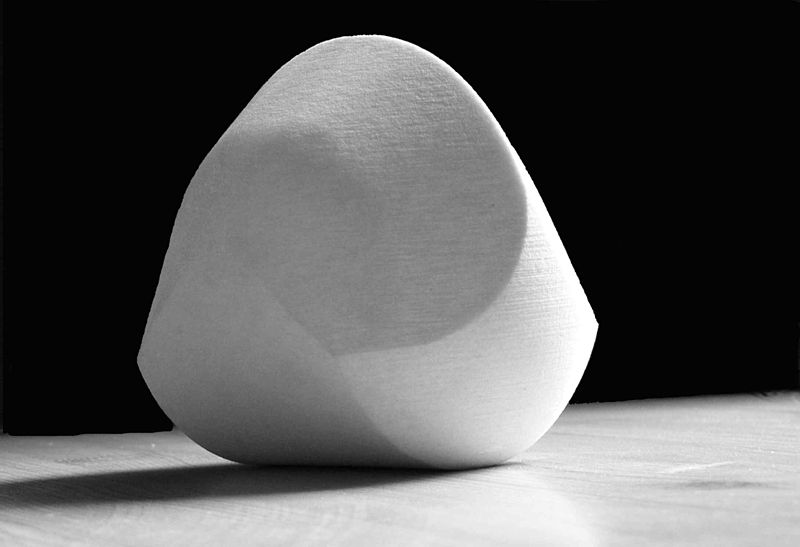
\includegraphics[scale=0.15]{Gomboc.jpg}
\caption{\label{fig:gomboc}Gömböc : un objet homogène tridimensionnel mono-monostatique. (source : Wikipedia)}
\end{figure}



\subsection{Codes}
Si vous souhaitez insérer du code dans votre rapport, invoquez les commandes : \\
 \texttt{\textbackslash lstset\{language=python\}}\\
 \texttt{\textbackslash lstinputlisting[caption=\{Titre du listing\}, label=\{lst:code\}]\{./code/code.py\}}


La première commande sélectionne le langage, pour que les mots clés de celui-ci soient correctement détectés et mis en valeur. 
La seconde commande permet d'insérer le code contenu dans le fichier code.py qui se trouve dans le sous-répertoire code.
Pour faire référence au code, il suffit de sélectionner le label du listing \ref{lst:prime},  comme pour les figures et les tableaux.

\lstset{language=python}
\lstinputlisting[caption={Titre du listing}, label={lst:prime}]{./code/primegen.py}


\subsection{Index et glossaire}

Pour insérer des entrées dans l'index, il suffit de déclarer des mots via la commande \texttt{\textbackslash index\{Fabrication d'un index\}} comme suit\footnote{Allez donc voir l'index \ref{sec:index} à la fin du document  !}. \index{Fabrication d'un index}

Pour utiliser le glossaire, il faut définir les termes dans le fichier \texttt{glossaire.tex} en utilisant la commande \texttt{\textbackslash newacronym\{label\}\{abbréviation\}\{Signification\}}. 
Puis,  \texttt{\textbackslash gls\{label\}} permet de les utiliser dans le document. 


Par exemple, les UVs 3.4 et 4.4 sont une initiation à l'\gls{IS}. 
Un concept de gestion de projet souvent mal connu est le \gls{WBS}.


\section{Références bibliographiques}

Les références bibliographiques sont des documents numériques, des livres, des articles, des images ou des vidéos qui ne sont pas présents dans le rapport. 
\LaTeX propose un mécanisme simple de citation.
Pour plus de détails, vous pouvez consulter les références suivantes \cite{maguis2010redigez,desgraupes2003latex,bitouze2010latex} qui sont présentent à la médiathèque de l'ENSTA Bretagne, ou celle-ci directement sur le web \cite{openclassroomLaTeX}.  

Pour citer des documents, il suffit d'appeler la commande \texttt{\textbackslash cite\{key\}} en choisissant la clé qui identifie le document, comme suit : \cite{lamport1985i1}. 
Cette clé de citation est celle qui référence l'ouvrage dans le fichier de bibliographie intitulé   \texttt{bibliographie.bib}.
Ce fichier d'exemple contient tous les types de documents dont vous aurez besoin : livre, article de journal, références web,  rapport\dots 
Une fois insérée et compilée, la citation devient un lien dans le fichier pdf, redirigeant ainsi directement vers le détail de l'ouvrage cité dans la bibliographie située à la fin du document.
 

\mainmatter       % La partie principale du document

%----------------------------------------------------------------------------------------
%	PART I 
%----------------------------------------------------------------------------------------
\part{Introduction au projet}
\chapter{Formulation initiale du projet}



\section{Contexte}

BeeHive Monitoring System (BMONS) est un projet qui a pour but d'aider les apiculteurs. Il s'agit de leur proposer un système de surveillance et de détection peu onéreux afin de prodiguer les meilleurs soins au meilleur moment aux ruches qui en ont besoin et d'éviter les vols.

En effet, les abeilles sont vitales à l'équilibre écologique. Einstein avait même dit: " Si l’abeille disparaît, l’humanité en a pour quatre ans à vivre ". Sans elles 84 \% des espèces végétales cultivées pour l'alimentation disparaitraient. Or les abeilles sauvages sont aujourd'hui rares et l'espèce ne survivrai pas sans l'aide des apiculteurs. Ainsi le travail de ces derniers est crucial non seulement pour assurer la production de miel mais aussi pour la sauvegarde de l'environnement. Cependant, ces dernières années, les apiculteurs ont été confrontés à de nombreux problèmes et nous sommes aujourd'hui face à une diminution du nombre d'abeilles telles que la production annuelle européenne de miel est quatre fois moindre que celle d'il y a vingt ans. 

Pour aider à la résolution de ce problème, nous voulons donc créer un système capable d'aider l'apiculteur dans son travail et de ce fait combattre la disparition des abeilles. 

\section{Expression initiale du besoin}

Après avoir discuté avec plusieurs apiculteurs, nous avons pu identifier leurs besoins et déterminer de quelle manière nous pouvons les aider. Ainsi l'objectif de ce système est tout d'abord de donner accès à l'apiculteur à des informations clés sur la ruche sans que celui-ci n'ai à se déplacer, ni à ouvrir les ruches. En effet l'ouverture de la ruche perturbe les abeilles et elle n'est pas possible en hiver à cause des températures trop basses. De plus les ruches sont souvent disposées dans des ruchers éloignés les uns des autres, ce qui complique le travail de l'apiculteur. Les informations nécessaires seraient : la température dans et en dehors de la ruche, le poids, l'humidité et les sons de la ruches. Mais le système devra aussi alerter l'apiculteur quand la sécurité de la ruche est compromise, pour permettre une action rapide destinée à sauver la colonie.

Le système BMONS est donc composé de deux parties distinctes. La première consiste en un élément embarqué dans la ruche qui consomme un minimum d'énergie et qui mesure les paramètres clés. Les données de cet élément embarqué sont transmises à un serveur via un transmetteur sans fils à un serveur qui constitue la deuxième partie du système. Il donne accès à l'apiculteur aux différentes mesures effectuées dans et autour des ruches. Il envoie également des alertes de sécurités à l'apiculteur si besoin. 
\input{GANTT}


%----------------------------------------------------------------------------------------
%	PART II 
%----------------------------------------------------------------------------------------
\part{Notre plan}

\chapter{Architecture physique}

\section{Architecture physique}

\input{TestUnitaire}

%----------------------------------------------------------------------------------------
%	PART III 
%----------------------------------------------------------------------------------------
\part{Comment on vas s'y prendre}
\input{Strategie}
\chapter{Intégration}



%----------------------------------------------------------------------------------------
%	PART IV 
%----------------------------------------------------------------------------------------
\part{Qu'est ce que ça donne}
\input{EcartFonctionnel}
\input{BilanVFU}

%----------------------------------------------------------------------------------------
%	PART V 
%----------------------------------------------------------------------------------------
\part{Futur ?}
\input{Perspective}
\chapter{Conclusion}\\
Le projet BMONS a pour ambition de réaliser un système embarqué sur une ruche pour récolter les paramètres physiques de la ruche dans l’optique de détecter les anomalies de comportement des abeilles. Notre équipe s’est donc penché sur cette problématique avec des notions d’apiculture et de conduite de projet plutôt minces.

Après la première partie du projet nous pouvons enfin dire que nous comprenons les besoins et les attentes des apiculteurs, par exemple des fonctions auxquelles nous avions pensé, comme la détection du taux d'humidité dans la ruche ne semblent finalement pas primordiale au projet. En revanche des options comme le comptage des abeilles seraient appréciées par les apiculteurs, mais des compromis doivent êtres faits car certaines de ces options entrainent un surcoût trop conséquent pour que le projet satisfasse les exigences initiales.\newline 

Nous devons une grande partie de ces connaissances en apiculture aux réponses précises de monsieur Franck Singhoff, qui nous a également prêté une ruche pour que nous puissions travailler sur l'implémentation des capteurs sur notre prototype. \newline 

Les difficultés que nous avons rencontrées, par exemple lors de la compréhension et de la création des diagrammes nécessaires à l'établissement de la spécification fonctionnelle sur les trois axes, ont été surmontées grâce à l’aide de nos encadrants de projet, mais aussi grâce au dialogue entre les membres du groupe. Les choix des divers composants qui constitueront le prototype ont aussi été une source de problèmes, car même si nous avions une idée de quel type de composant nous avions besoin, faire le tri entre tous ceux qui existent nécessite de faire des choix entre par exemple le prix et la précision d’un capteur, et cela influe sur les exigences du projet. Enfin, la mise en place du serveur et de la création du cadre de mesure nous a permis d'acquérir des connaissances en protocole HTTP et en programmation Arduino. Nous avons pu ainsi être confronté aux problèmes de la communication sans fil.\newline

Ces quelques mois de travail en commun nous ont permis d'avoir un aperçu d'ensemble de la conduite d'un projet. Nous nous sommes rendu compte de la quantité de travail que représente la partie ingénierie système sur un projet comme celui-ci. Néanmoins, cette partie nous a permis de mieux anticiper l'intégration des capteurs et nous a donné une meilleure vision de la gestion de la base de données. 






\appendix
\part{Annexes}
 

\backmatter % Partie finale du document, non numérotée

%----------------------------------------------------------------------------------------
%	BIBLIOGRAPHIE
%----------------------------------------------------------------------------------------
%\addcontentsline{toc}{part}{Bibliographie}
%\bibliographystyle{apalike-fr}
%\bibliographystyle{plain-fr}
%\bibliography{bibliographie}
%\nocite{*}

%----------------------------------------------------------------------------------------
%	INDEX
%----------------------------------------------------------------------------------------
\cleardoublepage
\phantomsection
\setlength{\columnsep}{0.75cm}
\addcontentsline{toc}{part}{Index}
\label{sec:index}
\printindex

%----------------------------------------------------------------------------------------
%	GLOSSAIRE
%----------------------------------------------------------------------------------------
\cleardoublepage
\phantomsection
\setlength{\columnsep}{0.75cm}
\addcontentsline{toc}{part}{Glossaire}
\printglossaries

%----------------------------------------------------------------------------------------

\end{document}